\documentclass[]{article}
\usepackage{lmodern}
\usepackage{amssymb,amsmath}
\usepackage{ifxetex,ifluatex}
\usepackage{fixltx2e} % provides \textsubscript
\ifnum 0\ifxetex 1\fi\ifluatex 1\fi=0 % if pdftex
  \usepackage[T1]{fontenc}
  \usepackage[utf8]{inputenc}
\else % if luatex or xelatex
  \ifxetex
    \usepackage{mathspec}
  \else
    \usepackage{fontspec}
  \fi
  \defaultfontfeatures{Ligatures=TeX,Scale=MatchLowercase}
\fi
% use upquote if available, for straight quotes in verbatim environments
\IfFileExists{upquote.sty}{\usepackage{upquote}}{}
% use microtype if available
\IfFileExists{microtype.sty}{%
\usepackage{microtype}
\UseMicrotypeSet[protrusion]{basicmath} % disable protrusion for tt fonts
}{}
\usepackage[margin=1in]{geometry}
\usepackage{hyperref}
\hypersetup{unicode=true,
            pdftitle={Implementing K-Means},
            pdfauthor={Gabriel Ndoum},
            pdfborder={0 0 0},
            breaklinks=true}
\urlstyle{same}  % don't use monospace font for urls
\usepackage{color}
\usepackage{fancyvrb}
\newcommand{\VerbBar}{|}
\newcommand{\VERB}{\Verb[commandchars=\\\{\}]}
\DefineVerbatimEnvironment{Highlighting}{Verbatim}{commandchars=\\\{\}}
% Add ',fontsize=\small' for more characters per line
\usepackage{framed}
\definecolor{shadecolor}{RGB}{248,248,248}
\newenvironment{Shaded}{\begin{snugshade}}{\end{snugshade}}
\newcommand{\KeywordTok}[1]{\textcolor[rgb]{0.13,0.29,0.53}{\textbf{#1}}}
\newcommand{\DataTypeTok}[1]{\textcolor[rgb]{0.13,0.29,0.53}{#1}}
\newcommand{\DecValTok}[1]{\textcolor[rgb]{0.00,0.00,0.81}{#1}}
\newcommand{\BaseNTok}[1]{\textcolor[rgb]{0.00,0.00,0.81}{#1}}
\newcommand{\FloatTok}[1]{\textcolor[rgb]{0.00,0.00,0.81}{#1}}
\newcommand{\ConstantTok}[1]{\textcolor[rgb]{0.00,0.00,0.00}{#1}}
\newcommand{\CharTok}[1]{\textcolor[rgb]{0.31,0.60,0.02}{#1}}
\newcommand{\SpecialCharTok}[1]{\textcolor[rgb]{0.00,0.00,0.00}{#1}}
\newcommand{\StringTok}[1]{\textcolor[rgb]{0.31,0.60,0.02}{#1}}
\newcommand{\VerbatimStringTok}[1]{\textcolor[rgb]{0.31,0.60,0.02}{#1}}
\newcommand{\SpecialStringTok}[1]{\textcolor[rgb]{0.31,0.60,0.02}{#1}}
\newcommand{\ImportTok}[1]{#1}
\newcommand{\CommentTok}[1]{\textcolor[rgb]{0.56,0.35,0.01}{\textit{#1}}}
\newcommand{\DocumentationTok}[1]{\textcolor[rgb]{0.56,0.35,0.01}{\textbf{\textit{#1}}}}
\newcommand{\AnnotationTok}[1]{\textcolor[rgb]{0.56,0.35,0.01}{\textbf{\textit{#1}}}}
\newcommand{\CommentVarTok}[1]{\textcolor[rgb]{0.56,0.35,0.01}{\textbf{\textit{#1}}}}
\newcommand{\OtherTok}[1]{\textcolor[rgb]{0.56,0.35,0.01}{#1}}
\newcommand{\FunctionTok}[1]{\textcolor[rgb]{0.00,0.00,0.00}{#1}}
\newcommand{\VariableTok}[1]{\textcolor[rgb]{0.00,0.00,0.00}{#1}}
\newcommand{\ControlFlowTok}[1]{\textcolor[rgb]{0.13,0.29,0.53}{\textbf{#1}}}
\newcommand{\OperatorTok}[1]{\textcolor[rgb]{0.81,0.36,0.00}{\textbf{#1}}}
\newcommand{\BuiltInTok}[1]{#1}
\newcommand{\ExtensionTok}[1]{#1}
\newcommand{\PreprocessorTok}[1]{\textcolor[rgb]{0.56,0.35,0.01}{\textit{#1}}}
\newcommand{\AttributeTok}[1]{\textcolor[rgb]{0.77,0.63,0.00}{#1}}
\newcommand{\RegionMarkerTok}[1]{#1}
\newcommand{\InformationTok}[1]{\textcolor[rgb]{0.56,0.35,0.01}{\textbf{\textit{#1}}}}
\newcommand{\WarningTok}[1]{\textcolor[rgb]{0.56,0.35,0.01}{\textbf{\textit{#1}}}}
\newcommand{\AlertTok}[1]{\textcolor[rgb]{0.94,0.16,0.16}{#1}}
\newcommand{\ErrorTok}[1]{\textcolor[rgb]{0.64,0.00,0.00}{\textbf{#1}}}
\newcommand{\NormalTok}[1]{#1}
\usepackage{graphicx,grffile}
\makeatletter
\def\maxwidth{\ifdim\Gin@nat@width>\linewidth\linewidth\else\Gin@nat@width\fi}
\def\maxheight{\ifdim\Gin@nat@height>\textheight\textheight\else\Gin@nat@height\fi}
\makeatother
% Scale images if necessary, so that they will not overflow the page
% margins by default, and it is still possible to overwrite the defaults
% using explicit options in \includegraphics[width, height, ...]{}
\setkeys{Gin}{width=\maxwidth,height=\maxheight,keepaspectratio}
\IfFileExists{parskip.sty}{%
\usepackage{parskip}
}{% else
\setlength{\parindent}{0pt}
\setlength{\parskip}{6pt plus 2pt minus 1pt}
}
\setlength{\emergencystretch}{3em}  % prevent overfull lines
\providecommand{\tightlist}{%
  \setlength{\itemsep}{0pt}\setlength{\parskip}{0pt}}
\setcounter{secnumdepth}{0}
% Redefines (sub)paragraphs to behave more like sections
\ifx\paragraph\undefined\else
\let\oldparagraph\paragraph
\renewcommand{\paragraph}[1]{\oldparagraph{#1}\mbox{}}
\fi
\ifx\subparagraph\undefined\else
\let\oldsubparagraph\subparagraph
\renewcommand{\subparagraph}[1]{\oldsubparagraph{#1}\mbox{}}
\fi

%%% Use protect on footnotes to avoid problems with footnotes in titles
\let\rmarkdownfootnote\footnote%
\def\footnote{\protect\rmarkdownfootnote}

%%% Change title format to be more compact
\usepackage{titling}

% Create subtitle command for use in maketitle
\providecommand{\subtitle}[1]{
  \posttitle{
    \begin{center}\large#1\end{center}
    }
}

\setlength{\droptitle}{-2em}

  \title{Implementing K-Means}
    \pretitle{\vspace{\droptitle}\centering\huge}
  \posttitle{\par}
    \author{Gabriel Ndoum}
    \preauthor{\centering\large\emph}
  \postauthor{\par}
      \predate{\centering\large\emph}
  \postdate{\par}
    \date{May 11, 2019}


\begin{document}
\maketitle

\begin{Shaded}
\begin{Highlighting}[]
\CommentTok{#let view the data then we can analyse.}
\NormalTok{crimeNaless <-}\StringTok{ }\KeywordTok{na.omit}\NormalTok{(USArrests)}
\NormalTok{crime <-}\StringTok{ }\KeywordTok{data.matrix}\NormalTok{(crimeNaless)}
\KeywordTok{str}\NormalTok{(crime)}
\end{Highlighting}
\end{Shaded}

\begin{verbatim}
##  num [1:50, 1:4] 13.2 10 8.1 8.8 9 7.9 3.3 5.9 15.4 17.4 ...
##  - attr(*, "dimnames")=List of 2
##   ..$ : chr [1:50] "Alabama" "Alaska" "Arizona" "Arkansas" ...
##   ..$ : chr [1:4] "Murder" "Assault" "UrbanPop" "Rape"
\end{verbatim}

\begin{Shaded}
\begin{Highlighting}[]
\NormalTok{crime}
\end{Highlighting}
\end{Shaded}

\begin{verbatim}
##                Murder Assault UrbanPop Rape
## Alabama          13.2     236       58 21.2
## Alaska           10.0     263       48 44.5
## Arizona           8.1     294       80 31.0
## Arkansas          8.8     190       50 19.5
## California        9.0     276       91 40.6
## Colorado          7.9     204       78 38.7
## Connecticut       3.3     110       77 11.1
## Delaware          5.9     238       72 15.8
## Florida          15.4     335       80 31.9
## Georgia          17.4     211       60 25.8
## Hawaii            5.3      46       83 20.2
## Idaho             2.6     120       54 14.2
## Illinois         10.4     249       83 24.0
## Indiana           7.2     113       65 21.0
## Iowa              2.2      56       57 11.3
## Kansas            6.0     115       66 18.0
## Kentucky          9.7     109       52 16.3
## Louisiana        15.4     249       66 22.2
## Maine             2.1      83       51  7.8
## Maryland         11.3     300       67 27.8
## Massachusetts     4.4     149       85 16.3
## Michigan         12.1     255       74 35.1
## Minnesota         2.7      72       66 14.9
## Mississippi      16.1     259       44 17.1
## Missouri          9.0     178       70 28.2
## Montana           6.0     109       53 16.4
## Nebraska          4.3     102       62 16.5
## Nevada           12.2     252       81 46.0
## New Hampshire     2.1      57       56  9.5
## New Jersey        7.4     159       89 18.8
## New Mexico       11.4     285       70 32.1
## New York         11.1     254       86 26.1
## North Carolina   13.0     337       45 16.1
## North Dakota      0.8      45       44  7.3
## Ohio              7.3     120       75 21.4
## Oklahoma          6.6     151       68 20.0
## Oregon            4.9     159       67 29.3
## Pennsylvania      6.3     106       72 14.9
## Rhode Island      3.4     174       87  8.3
## South Carolina   14.4     279       48 22.5
## South Dakota      3.8      86       45 12.8
## Tennessee        13.2     188       59 26.9
## Texas            12.7     201       80 25.5
## Utah              3.2     120       80 22.9
## Vermont           2.2      48       32 11.2
## Virginia          8.5     156       63 20.7
## Washington        4.0     145       73 26.2
## West Virginia     5.7      81       39  9.3
## Wisconsin         2.6      53       66 10.8
## Wyoming           6.8     161       60 15.6
\end{verbatim}

\begin{Shaded}
\begin{Highlighting}[]
\CommentTok{# will choose 5 as the number of cluster. The syntax is : kmeans( data, k) }
\CommentTok{# where k is the number of cluster centers.}
\NormalTok{cluster <-}\StringTok{ }\KeywordTok{kmeans}\NormalTok{(crime,}\DecValTok{5}\NormalTok{)}
\KeywordTok{class}\NormalTok{(cluster)}
\end{Highlighting}
\end{Shaded}

\begin{verbatim}
## [1] "kmeans"
\end{verbatim}

\begin{Shaded}
\begin{Highlighting}[]
\CommentTok{#let's analyse the clustering}
\KeywordTok{str}\NormalTok{(cluster)}
\end{Highlighting}
\end{Shaded}

\begin{verbatim}
## List of 9
##  $ cluster     : Named int [1:50] 3 3 2 4 3 4 1 3 2 4 ...
##   ..- attr(*, "names")= chr [1:50] "Alabama" "Alaska" "Arizona" "Arkansas" ...
##  $ centers     : num [1:5, 1:4] 5.59 11.95 11.77 8.21 2.95 ...
##   ..- attr(*, "dimnames")=List of 2
##   .. ..$ : chr [1:5] "1" "2" "3" "4" ...
##   .. ..$ : chr [1:4] "Murder" "Assault" "UrbanPop" "Rape"
##  $ totss       : num 355808
##  $ withinss    : num [1:5] 1480 2546 6706 9137 4548
##  $ tot.withinss: num 24417
##  $ betweenss   : num 331391
##  $ size        : int [1:5] 10 4 12 14 10
##  $ iter        : int 2
##  $ ifault      : int 0
##  - attr(*, "class")= chr "kmeans"
\end{verbatim}

\begin{Shaded}
\begin{Highlighting}[]
\CommentTok{#the str() function gives the structure of the kmeans with the following parameters:}
\CommentTok{#withinss, betweenss, etc, analyzing which you can find out the performance of kmeans.}

\CommentTok{#betweenss : Between sum of squares for instance Intracluster similarity}

\CommentTok{#withinss : Within sum of square such as Intercluster similarity}

\CommentTok{#totwithinss : Sum of all the withinss of all the clusters : Total intra-cluster similarity}

\CommentTok{#Let see how we can find the optimal value of 'k'.}

\CommentTok{# Dissortion : can be calculated in terms of withinss.}
\CommentTok{# Lesser the value of 'withinss' of a particular cluster,}
\CommentTok{# more densely populated it will be, thus minimum distortion}
\CommentTok{#This function takes up the data and the value of k }
\CommentTok{#and returns the 'km$totwithinss' for it}
\NormalTok{kmeans.wss.k <-}\StringTok{ }\ControlFlowTok{function}\NormalTok{(crime, k)\{}
\NormalTok{  km =}\StringTok{ }\KeywordTok{kmeans}\NormalTok{(crime, k)}
  \KeywordTok{return}\NormalTok{ (km}\OperatorTok{$}\NormalTok{tot.withinss)}
\NormalTok{\}}

\KeywordTok{kmeans.wss.k}\NormalTok{(crime,}\DecValTok{5}\NormalTok{) }\CommentTok{# what is the value of withinss for k=5}
\end{Highlighting}
\end{Shaded}

\begin{verbatim}
## [1] 32961.6
\end{verbatim}

\begin{Shaded}
\begin{Highlighting}[]
\CommentTok{# lets increase k value. let go with 10}
\KeywordTok{kmeans.wss.k}\NormalTok{(crime,}\DecValTok{10}\NormalTok{)}
\end{Highlighting}
\end{Shaded}

\begin{verbatim}
## [1] 10184.86
\end{verbatim}

\begin{Shaded}
\begin{Highlighting}[]
\CommentTok{#It can be seen that as the value of K increases, distortion decreases.}

\CommentTok{#We can take out the different values of 'km$totwithinss' }
\CommentTok{#and plot them in a graph to find the relationship }
\CommentTok{#between distortion and the value of k. }
\CommentTok{#The following function does that for us:}
\NormalTok{kmeans.dis <-}\StringTok{ }\ControlFlowTok{function}\NormalTok{(crime, maxk)\{}
\NormalTok{  dis=(}\KeywordTok{nrow}\NormalTok{(crime)}\OperatorTok{-}\DecValTok{1}\NormalTok{)}\OperatorTok{*}\KeywordTok{sum}\NormalTok{(}\KeywordTok{apply}\NormalTok{(crime,}\DecValTok{2}\NormalTok{,var))}
\NormalTok{  dis[}\DecValTok{2}\OperatorTok{:}\NormalTok{maxk]=}\KeywordTok{sapply}\NormalTok{ (}\DecValTok{2}\OperatorTok{:}\NormalTok{maxk, kmeans.wss.k, }\DataTypeTok{crime=}\NormalTok{crime)}
  \KeywordTok{return}\NormalTok{(dis)}
\NormalTok{\}}
\NormalTok{maxk =}\StringTok{ }\DecValTok{10}
\NormalTok{dis =}\StringTok{ }\KeywordTok{kmeans.dis}\NormalTok{(crime, maxk);}
\KeywordTok{plot}\NormalTok{(}\DecValTok{1}\OperatorTok{:}\NormalTok{maxk, dis, }\DataTypeTok{type=}\StringTok{'b'}\NormalTok{, }\DataTypeTok{xlab=}\StringTok{"Number of Clusters"}\NormalTok{,}
     \DataTypeTok{ylab=}\StringTok{"Distortion"}\NormalTok{,}
     \DataTypeTok{col=}\StringTok{"red"}\NormalTok{)}
\end{Highlighting}
\end{Shaded}

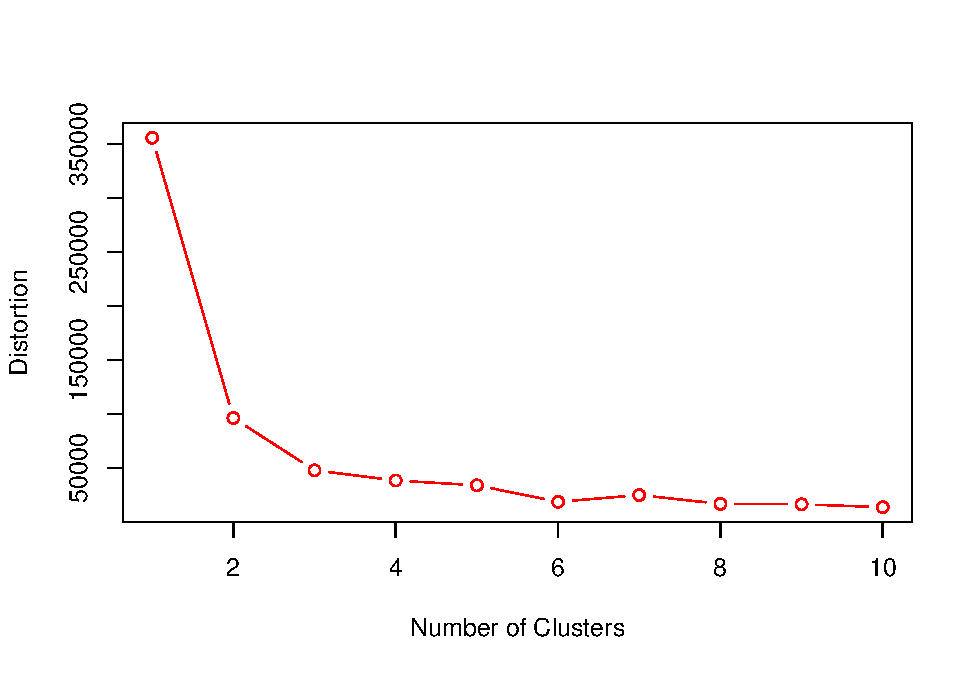
\includegraphics{Imlementing_K-Means_Clustering_with_R_files/figure-latex/unnamed-chunk-1-1.pdf}

\begin{Shaded}
\begin{Highlighting}[]
\CommentTok{#Elbow Curve: This is the plot between 'k', the number of clusters }
\CommentTok{#and the 'totwithinss' (or distortion) for each value of k. }
\CommentTok{#With less cluster, there is a significant decrease in distortion too. }
\CommentTok{#This value of k(4) beyond which the distortion rate becomes constant is the optimal value}

\CommentTok{#Let us apply some animation to understand how R gave us the clustered results.}

\KeywordTok{library}\NormalTok{(animation)}
\NormalTok{cluster<-}\StringTok{ }\KeywordTok{kmeans.ani}\NormalTok{(crime, }\DecValTok{4}\NormalTok{)}
\end{Highlighting}
\end{Shaded}

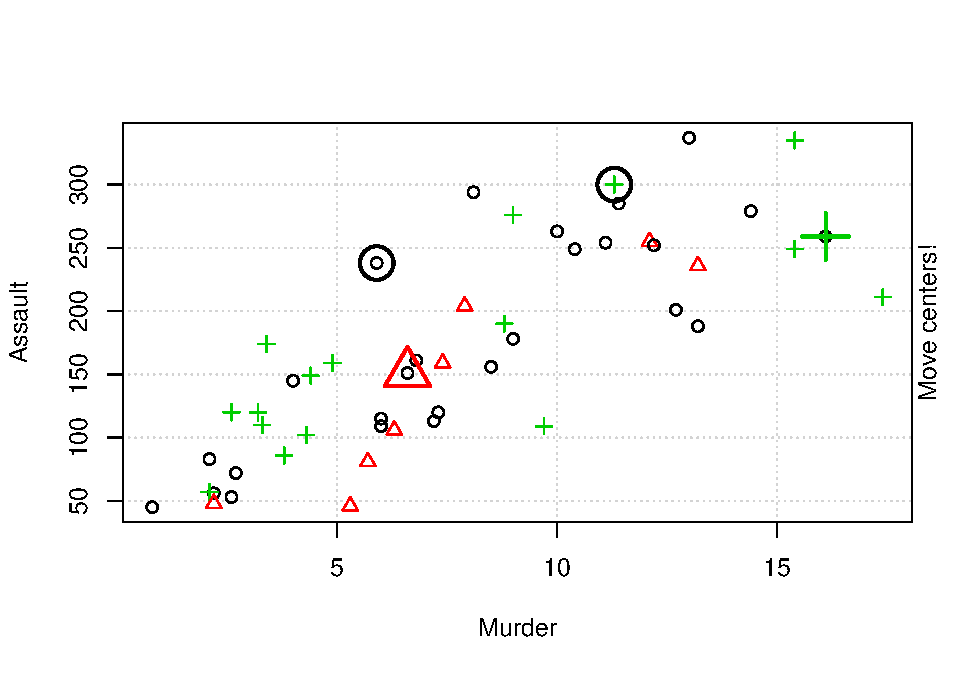
\includegraphics{Imlementing_K-Means_Clustering_with_R_files/figure-latex/unnamed-chunk-1-2.pdf}
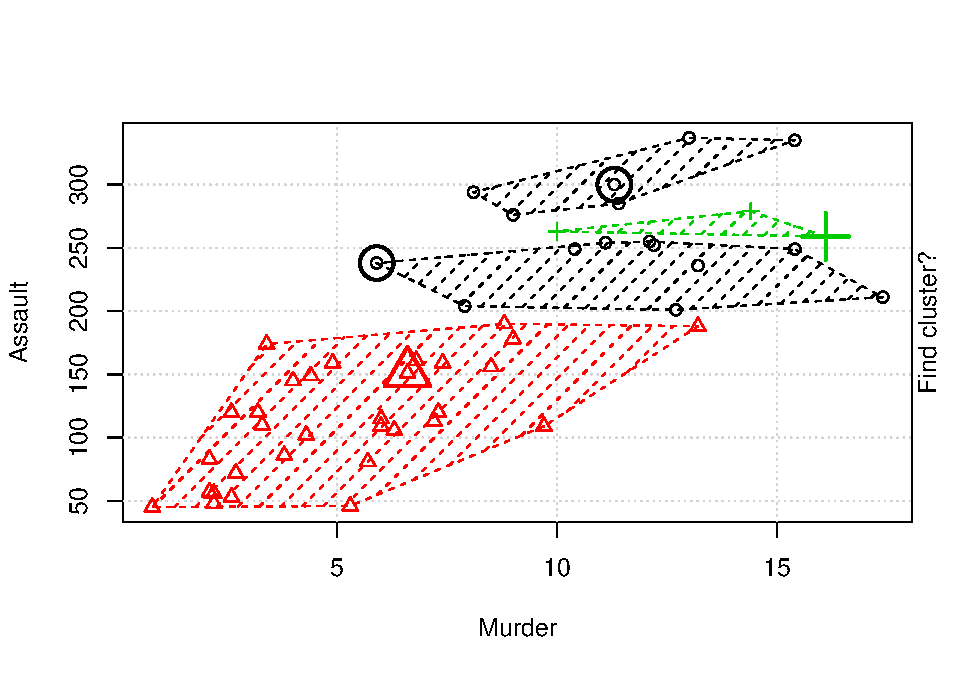
\includegraphics{Imlementing_K-Means_Clustering_with_R_files/figure-latex/unnamed-chunk-1-3.pdf}
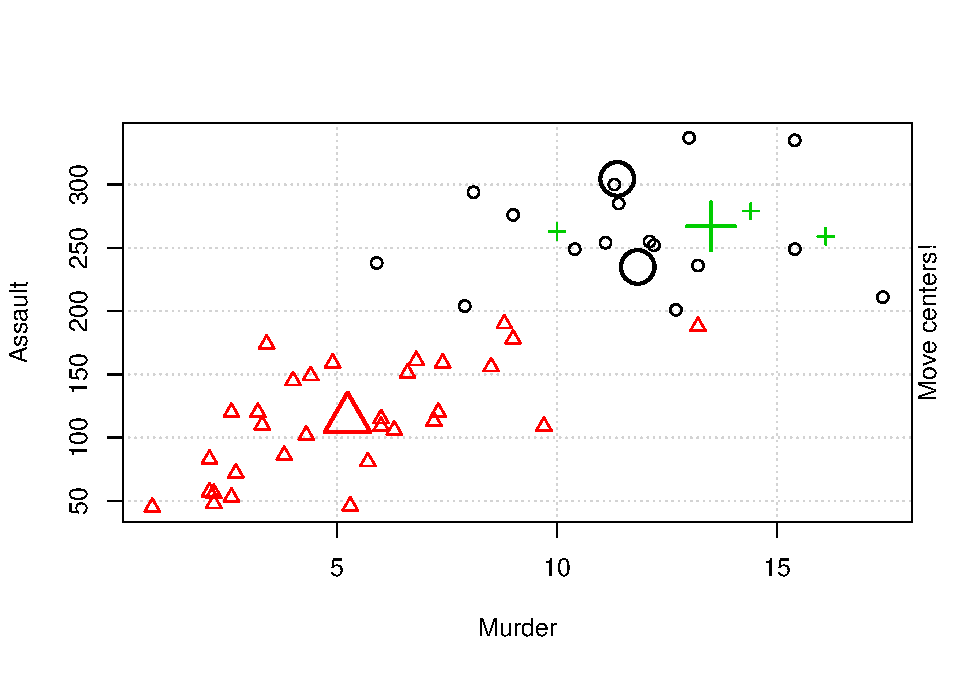
\includegraphics{Imlementing_K-Means_Clustering_with_R_files/figure-latex/unnamed-chunk-1-4.pdf}
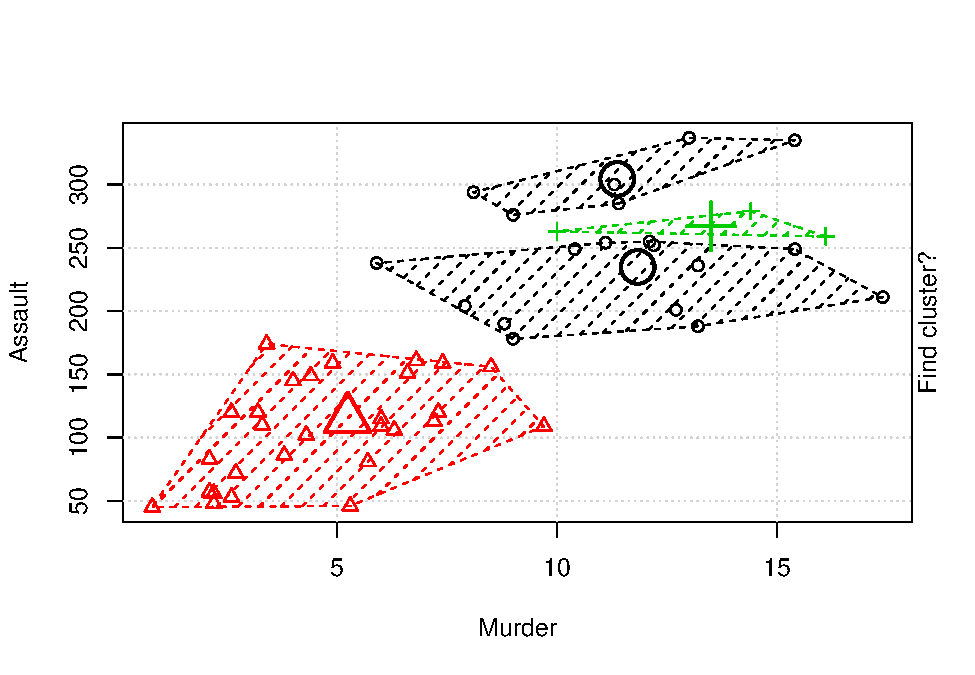
\includegraphics{Imlementing_K-Means_Clustering_with_R_files/figure-latex/unnamed-chunk-1-5.pdf}
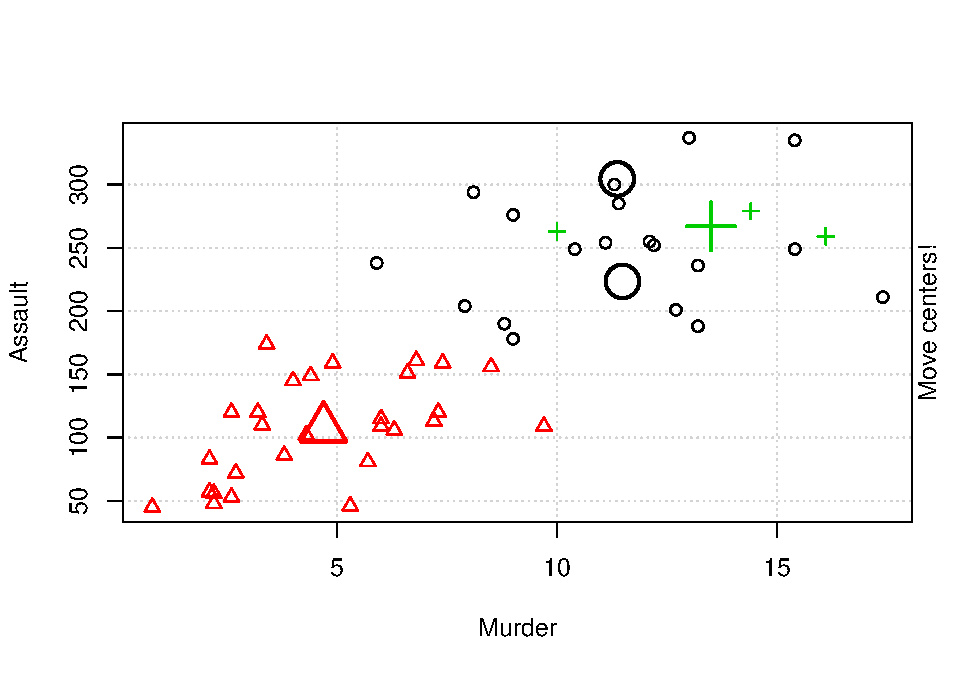
\includegraphics{Imlementing_K-Means_Clustering_with_R_files/figure-latex/unnamed-chunk-1-6.pdf}
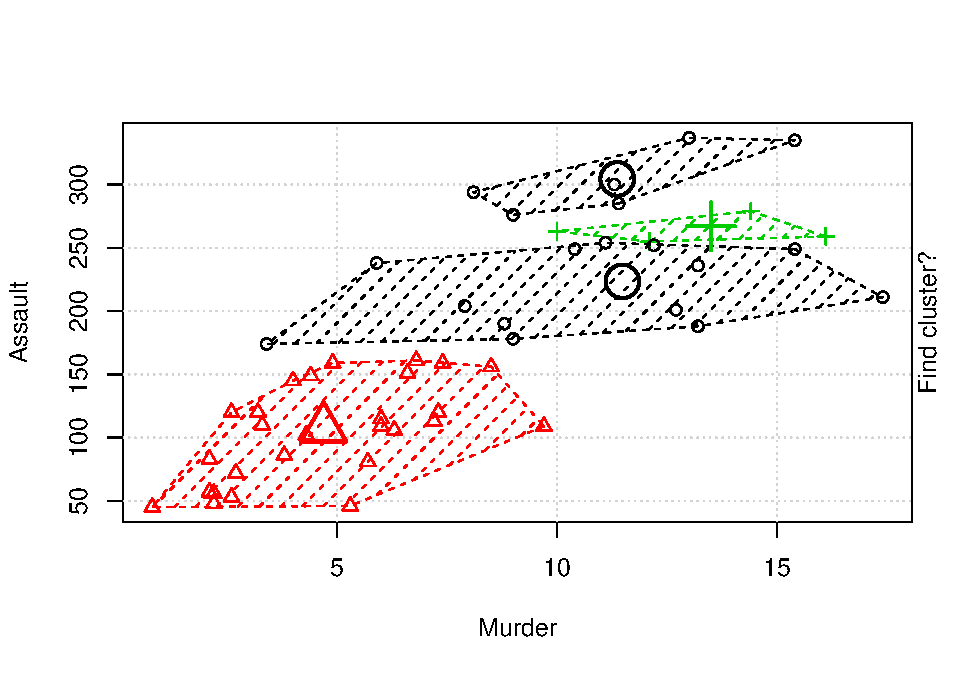
\includegraphics{Imlementing_K-Means_Clustering_with_R_files/figure-latex/unnamed-chunk-1-7.pdf}
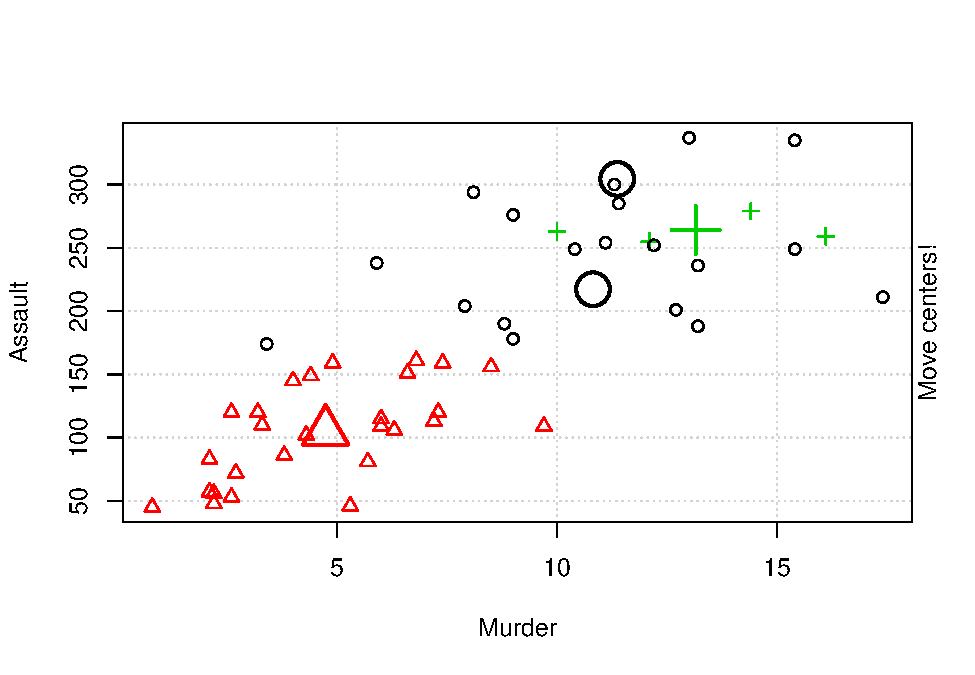
\includegraphics{Imlementing_K-Means_Clustering_with_R_files/figure-latex/unnamed-chunk-1-8.pdf}
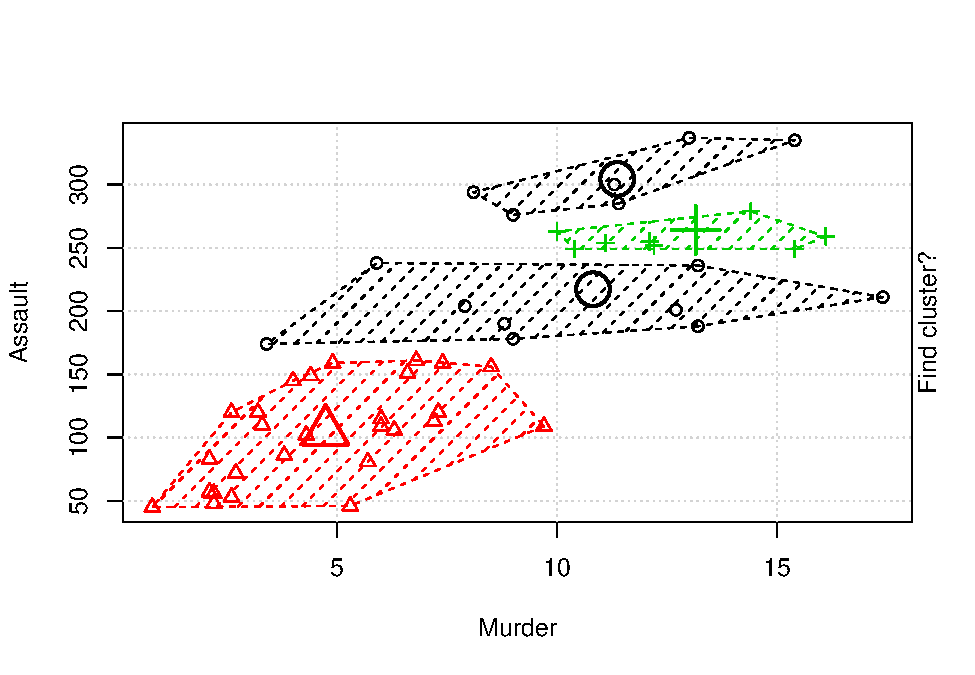
\includegraphics{Imlementing_K-Means_Clustering_with_R_files/figure-latex/unnamed-chunk-1-9.pdf}
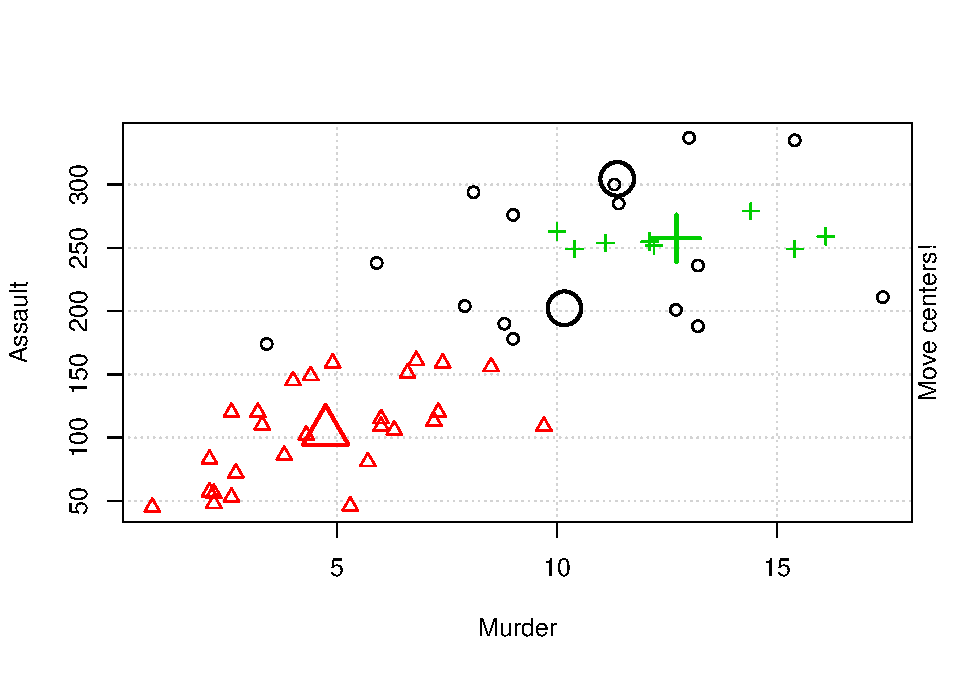
\includegraphics{Imlementing_K-Means_Clustering_with_R_files/figure-latex/unnamed-chunk-1-10.pdf}
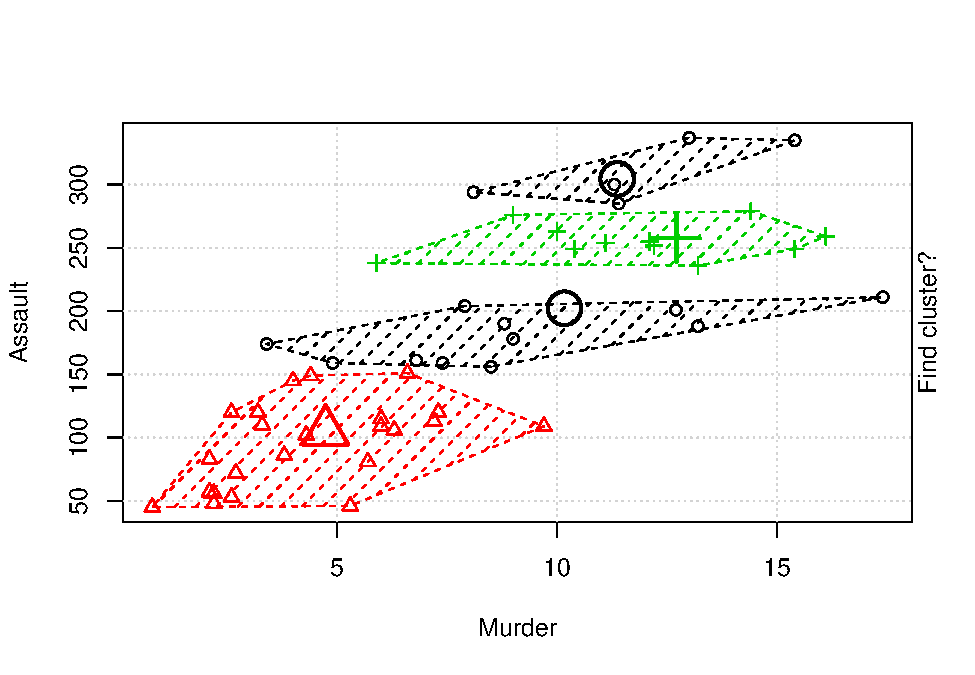
\includegraphics{Imlementing_K-Means_Clustering_with_R_files/figure-latex/unnamed-chunk-1-11.pdf}
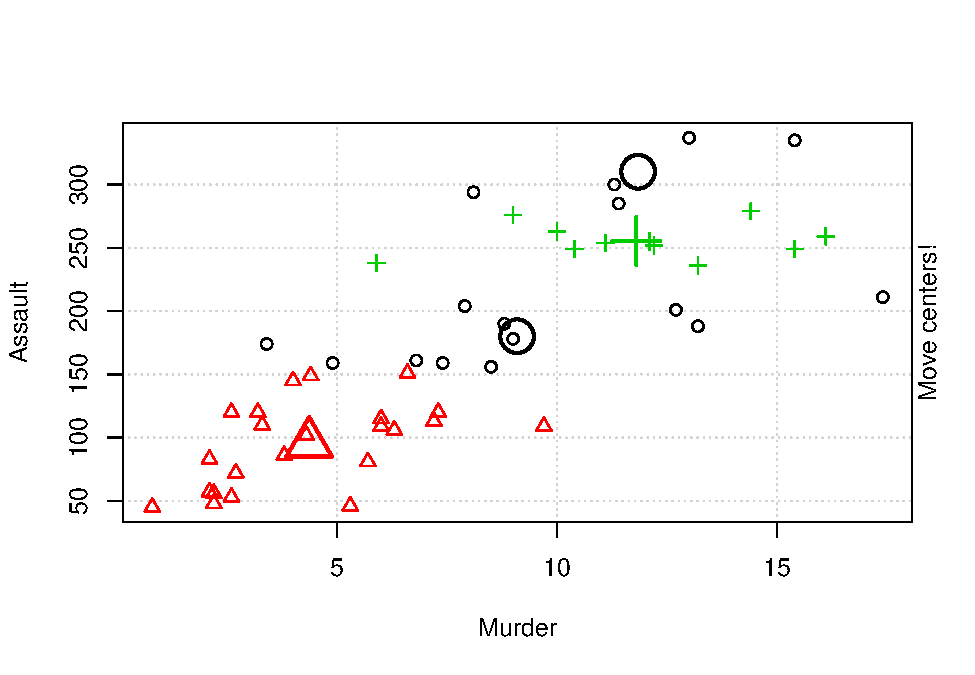
\includegraphics{Imlementing_K-Means_Clustering_with_R_files/figure-latex/unnamed-chunk-1-12.pdf}
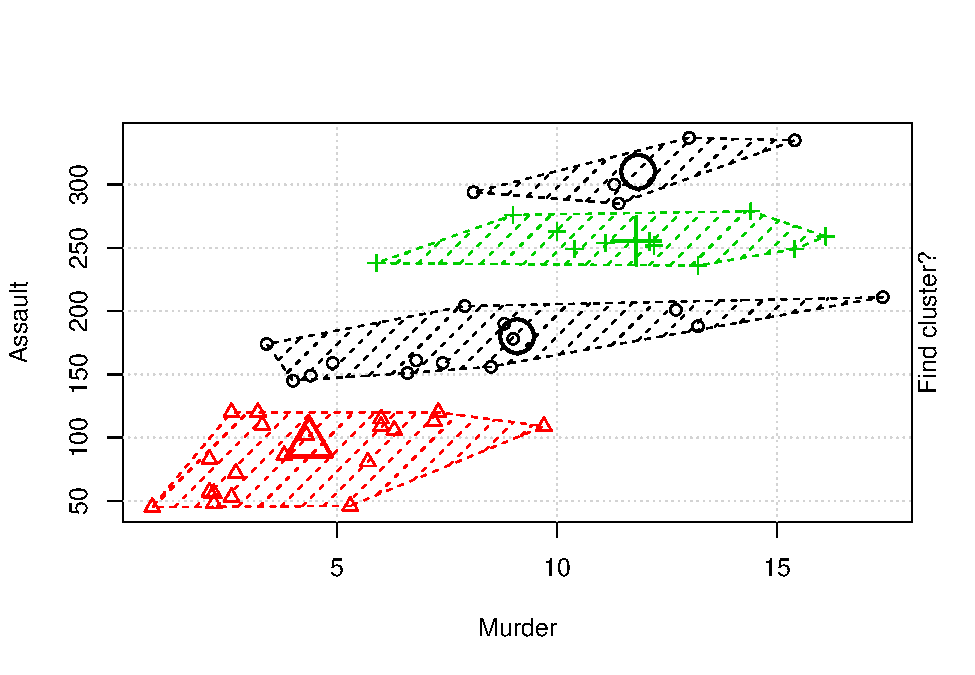
\includegraphics{Imlementing_K-Means_Clustering_with_R_files/figure-latex/unnamed-chunk-1-13.pdf}
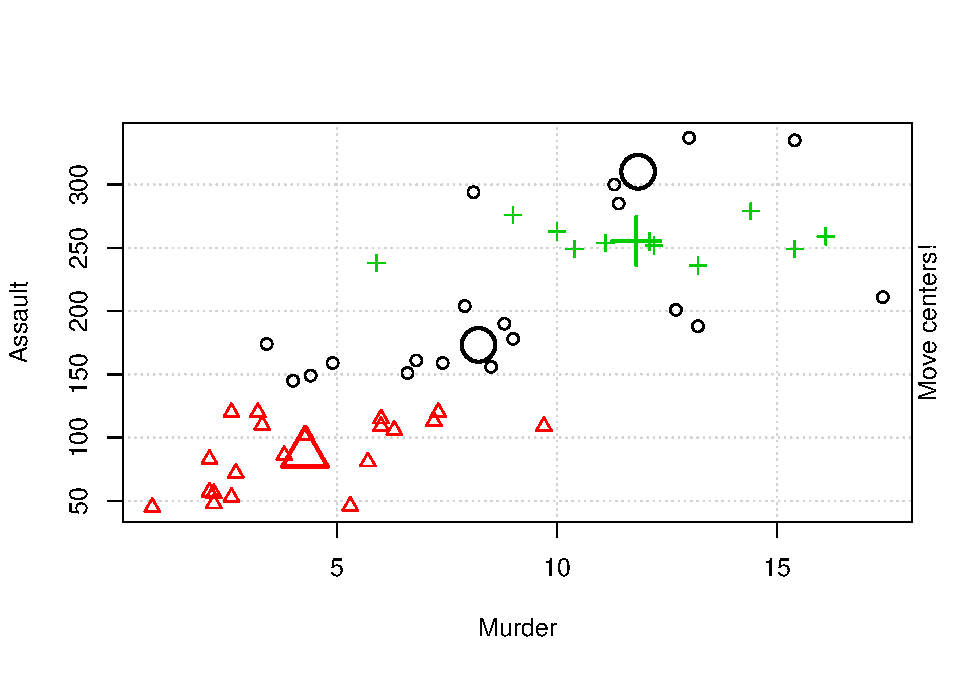
\includegraphics{Imlementing_K-Means_Clustering_with_R_files/figure-latex/unnamed-chunk-1-14.pdf}
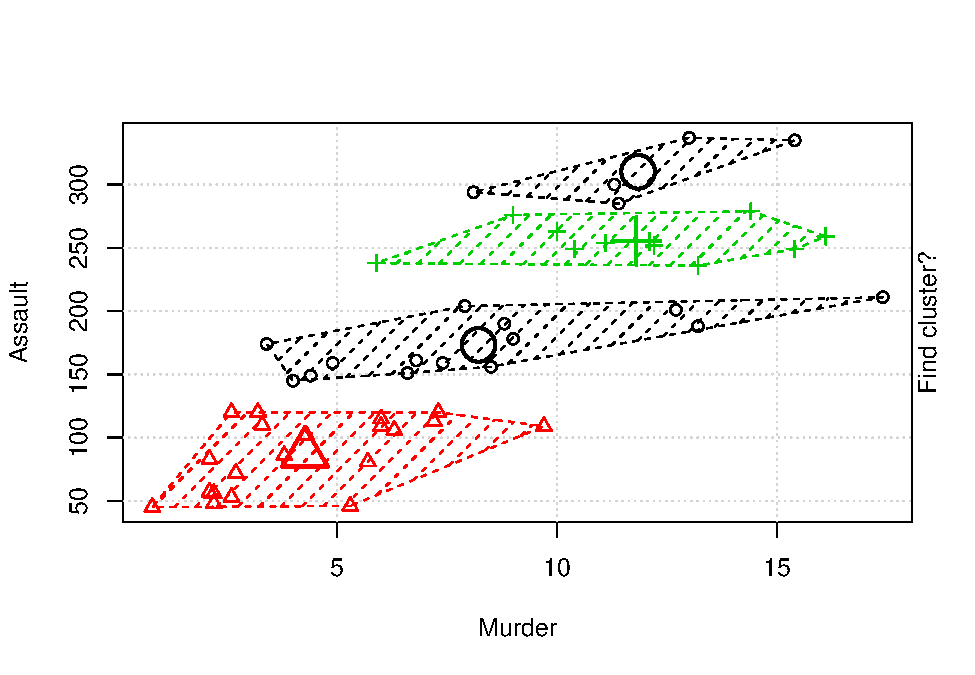
\includegraphics{Imlementing_K-Means_Clustering_with_R_files/figure-latex/unnamed-chunk-1-15.pdf}

\begin{Shaded}
\begin{Highlighting}[]
\CommentTok{#The clustering accuracy can be determined by the animation chart of K-means clustering using }
\CommentTok{#the 'animation" package which shows the clustering process. }
\CommentTok{#If the clusters groups or centres aren't overlapping with each other we can conclude}
\CommentTok{#the clustering accuracy. We also can measure the accuracy of the new labelling by comparing it }
\CommentTok{#with the original labeling (original labelling is the ground truth) i.e using a table function}

\CommentTok{#It can be seen that the data is divided into 4 clusters. }
\CommentTok{# And the cluster centers are :}

\NormalTok{cluster}\OperatorTok{$}\NormalTok{centers}
\end{Highlighting}
\end{Shaded}

\begin{verbatim}
##                Murder  Assault UrbanPop     Rape
## Maryland    11.840000 310.2000 68.40000 27.78000
## Oklahoma     4.270000  87.5500 59.75000 14.39000
## Mississippi 11.800000 255.4545 68.27273 28.64545
## Delaware     8.214286 173.2857 70.64286 22.84286
\end{verbatim}

\begin{Shaded}
\begin{Highlighting}[]
\CommentTok{#Cluster-4 with 'Oregon' as the cluster center has a huge crime rate.}

\CommentTok{#Cluster-3 and Cluster-2 follow up.}
\end{Highlighting}
\end{Shaded}


\end{document}
